% meta.concepts: 3D force vector
% meta.tags: realistic
% acknowledge: Peter Seiler & Luke Melander graciously shared Spring 2019 course material
% source: 2019 P. Seiler AEM2011 HW 2

The space shuttle is headed in a direction that is $80^\circ$ relative to horizontal and $45^\circ$ west of north. The rocket thrust acts opposite the direction of travel of the space shuttle. Assume that the $x$, $y$, and $z$ coordinate axes are directed east, up, and south, respectively. 
\begin{enumerate}
  \item Draw the space shuttle and the assumed coordinate system.
  \item Determine the $x$, $y$, and $z$-components of the thrust force.
\end{enumerate}

% \vspace{.5cm}
% \rule{\textwidth}{.4pt}
% \vspace{.5cm}
% \textbf{Solution:}
% \begin{figure}[ht!]
%   \centering
%   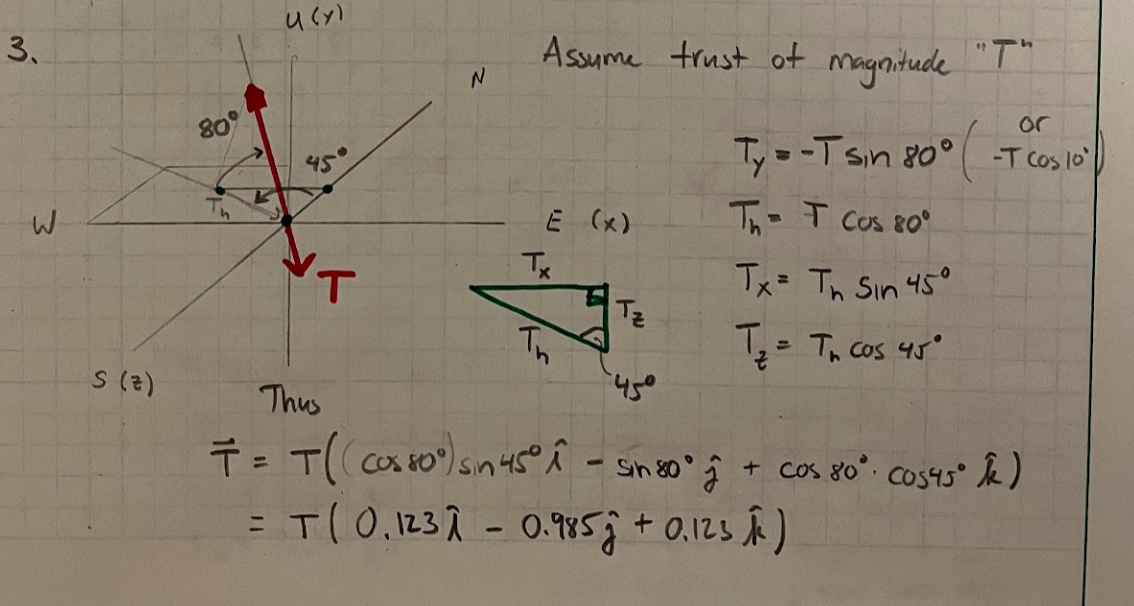
\includegraphics[width=0.9\textwidth]{soln.png}
% \end{figure}


